% Ch10 self-study -- "I do / You do" ladder for Zumdahl chapter 10.
% Twelve ladders, 48 questions, fourteen figures.
%
% SCOPE: unlike ch 9, almost all of this chapter is assessed --
% TEXTBOOK-MAP feeds 10.1-10.8 into CED 2.3, 2.4, 3.1, 3.2, 3.3 and 6.5.
% The skip list holds only "network solids DETAIL" (10.5) and phase
% diagrams (10.9), and the map calls 10.9 borderline: "not a CED topic,
% but a 20-minute treatment supports 3.3 and 6.5 well."  So network
% solids appear at working depth (not crystallographic detail) and phase
% diagrams get Ladder 12, labelled for what it is.
\documentclass{apchem-worksheet}

\apcunitword{Chapter}
\apcunit{10}
\apcunittitle{Liquids and Solids}
\apcdoctitle{Self-Study \textbullet\ Chapter 10, I~do / You~do}
\apcsubtitle{Zumdahl \S10.1--10.8 \textbullet\ PDF pp.\ 493--530}

\begin{document}
\apctitleblock

\begin{apcnote}[How to use these notes --- read this first]
Each skill is a \textbf{ladder}: a fully worked example in the
solid-framed box, then \textbf{four} YOUR TURN questions in the dashed
box --- same skill, new substances, no help. Work all four before
checking the gray \emph{check:} line; a tracker tick needs all four
right first time.

\textbf{This chapter is worth more than its size suggests.} Chapter 10
feeds \textbf{six} different CED topics, and Unit 3 --- your heaviest at
18--22\% of the exam --- draws on it directly. Nearly everything here is
assessed. Only Ladder 12 (phase diagrams) sits outside the CED, and it
is included because it explains the rest.

\textbf{The whole chapter in one sentence.} Everything a liquid or solid
does --- boils high or low, flows thick or thin, shatters or bends,
conducts or insulates --- follows from \emph{what holds its particles
together and how strongly}.

\textbf{The one habit that carries the whole chapter.} Before answering
anything, identify the \textbf{particles} and the \textbf{force between
them}. Ninety percent of Chapter 10 questions collapse the moment you do.
\end{apcnote}

% =====================================================================
\section*{\sffamily Ladder 1 \textbullet\ Identifying intermolecular
forces}
\zsec{10.1}

An intermolecular force acts \emph{between} particles. It is never the
bond \emph{inside} a molecule --- and confusing the two is the error
this chapter punishes hardest.

\begin{center}
\begin{tikzpicture}[font=\sffamily\footnotesize]
  % --- LDF ---
  \node[font=\sffamily\small\bfseries] at (1.5,3.15) {London dispersion};
  \node at (1.5,2.75) {\emph{all} particles};
  \fill[apcgray!25] (0.7,1.5) circle (0.42);
  \fill[apcgray!25] (2.3,1.5) circle (0.42);
  \node at (0.55,1.5) {\tiny $\delta-$}; \node at (0.9,1.5) {\tiny $\delta+$};
  \node at (2.15,1.5) {\tiny $\delta-$}; \node at (2.5,1.5) {\tiny $\delta+$};
  \draw[dotted,thick] (1.12,1.5) -- (1.88,1.5);
  \node[align=center] at (1.5,0.45)
    {a momentary lopsided cloud\\induces one next door};

  % --- dipole-dipole ---
  \begin{scope}[xshift=5.0cm]
    \node[font=\sffamily\small\bfseries] at (1.5,3.15) {dipole--dipole};
    \node at (1.5,2.75) {polar molecules};
    \draw[very thick] (0.35,1.5) -- (1.15,1.5);
    \fill (0.35,1.5) circle (0.09); \fill (1.15,1.5) circle (0.09);
    \node at (0.35,1.9) {\tiny $\delta+$}; \node at (1.15,1.9) {\tiny $\delta-$};
    \draw[very thick] (1.85,1.5) -- (2.65,1.5);
    \fill (1.85,1.5) circle (0.09); \fill (2.65,1.5) circle (0.09);
    \node at (1.85,1.9) {\tiny $\delta+$}; \node at (2.65,1.9) {\tiny $\delta-$};
    \draw[dotted,thick] (1.15,1.5) -- (1.85,1.5);
    \node[align=center] at (1.5,0.45)
      {permanent dipoles line up\\$\delta+$ to $\delta-$};
  \end{scope}

  % --- H-bond ---
  \begin{scope}[xshift=10.0cm]
    \node[font=\sffamily\small\bfseries] at (1.5,3.15) {hydrogen bond};
    \node at (1.5,2.75) {H on N, O or F};
    \node[font=\small] at (0.45,1.5) {O};
    \node[font=\small] at (1.15,1.5) {H};
    \draw[very thick] (0.62,1.5) -- (0.98,1.5);
    \node[font=\small] at (2.45,1.5) {O};
    \draw[dotted,very thick] (1.32,1.5) -- (2.28,1.5);
    \node at (0.45,1.92) {\tiny $\delta-$}; \node at (1.15,1.92) {\tiny $\delta+$};
    \node at (2.45,1.92) {\tiny $\delta-$};
    \node[align=center] at (1.5,0.45)
      {a special, very strong\\dipole--dipole case};
  \end{scope}
\end{tikzpicture}
\end{center}

\begin{apctrap}
\textbf{A hydrogen bond is not a bond.} It is an attraction
\emph{between} molecules, roughly \SI{20}{\kilo\joule\per\mole} --- about
one twentieth of the \SI{467}{\kilo\joule\per\mole} \ce{O-H} covalent
bond inside the molecule. When water boils, the hydrogen bonds break and
the \ce{O-H} bonds do not: steam is still \ce{H2O}. Any answer that has
covalent bonds breaking during a phase change is wrong.
\end{apctrap}

\begin{workedexample}[I do: name every force present]
\textbf{Rule first: every particle has London dispersion forces.} They
arise from momentary fluctuations in any electron cloud, so nothing is
exempt. The question is always \emph{what else} is present.

\textbf{(a) \ce{CH4}.} Tetrahedral, four identical \ce{C-H} bonds, bond
dipoles cancel $\Rightarrow$ nonpolar. \textbf{LDF only.}

\textbf{(b) \ce{CH3Cl}.} Tetrahedral but not symmetric --- one \ce{C-Cl}
bond is much more polar than the \ce{C-H} bonds, so the dipoles do not
cancel $\Rightarrow$ polar. \textbf{LDF $+$ dipole--dipole.}

\textbf{(c) \ce{CH3OH}.} Polar, and it has an \ce{H} attached directly to
\ce{O}. \textbf{LDF $+$ dipole--dipole $+$ hydrogen bonding.}

\textbf{(d) \ce{NaCl} dissolved in water.} \ce{Na+} and \ce{Cl-} ions
next to polar water molecules gives \textbf{ion--dipole}, the strongest
force in this family, and the reason ionic solids dissolve at all.

\textbf{The procedure, every time:} (1) LDF always. (2) Polar? add
dipole--dipole. (3) H on N, O or F? add hydrogen bonding. (4) Ions
present with a polar solvent? add ion--dipole.
\end{workedexample}

\begin{yourturn}[YOUR TURN 1 --- four questions]
Name \emph{every} intermolecular force present.
\begin{enumerate}[leftmargin=*,itemsep=0.5em]
  \item \ce{CO2} \workspace[1.4cm]
  \item \ce{NH3} \workspace[1.4cm]
  \item \ce{HCl} \workspace[1.4cm]
  \item \ce{CH3CH2OH} in water \workspace[1.6cm]
\end{enumerate}
\selfcheck{(a) LDF only \quad (b) LDF, dipole--dipole, H-bonding \quad
(c) LDF, dipole--dipole \quad (d) LDF, dipole--dipole, H-bonding}
\keyonly{\begin{apcanswer}(a) \textbf{LDF only.} \ce{CO2} is linear, so
its two bond dipoles cancel and the molecule is nonpolar --- polar bonds
do not guarantee a polar molecule. (b) \textbf{LDF, dipole--dipole and
hydrogen bonding}: trigonal pyramidal (so polar), with H bonded to N.
(c) \textbf{LDF and dipole--dipole}. There is no hydrogen bonding ---
\ce{Cl} is not N, O or F, despite being electronegative. (d)
\textbf{LDF, dipole--dipole and hydrogen bonding}, both between ethanol
molecules and between ethanol and water, since ethanol's \ce{-OH} can
both donate and accept.\end{apcanswer}}
\end{yourturn}

% =====================================================================
\section*{\sffamily Ladder 2 \textbullet\ Dispersion forces and
polarizability}
\zsec{10.1}

Dispersion forces are the weakest \emph{per contact} and yet they decide
most boiling points, because they grow with the size of the electron
cloud --- and clouds get large fast.

\begin{center}
\begin{tikzpicture}[font=\sffamily\footnotesize]
  \node[font=\sffamily\small\bfseries] at (1.2,2.75) {small atom};
  \fill[apcgray!45] (1.2,1.3) circle (0.4);
  \fill (1.2,1.3) circle (0.12);
  \node[align=center] at (1.2,0.25)
    {few electrons, held tightly\\\textbf{low} polarizability};

  \node[font=\sffamily\small\bfseries] at (5.4,2.75) {large atom};
  \fill[apcgray!30] (5.4,1.3) circle (0.85);
  \fill (5.4,1.3) circle (0.12);
  \node[align=center] at (5.4,0.25)
    {many electrons, held loosely\\\textbf{high} polarizability};

  % arrow stops at 7.9 and the text is anchored west at 8.2 -- centring
  % the text on 10.5 pushed its left edge back under the arrowhead.
  \draw[-{Stealth[length=3mm]},very thick] (6.7,1.3) -- (7.9,1.3);
  \node[anchor=west,align=left,font=\sffamily\footnotesize] at (8.2,1.3)
    {a loose cloud distorts more easily,\\
     so the momentary dipoles are bigger,\\
     so the dispersion force is \textbf{stronger}};
\end{tikzpicture}
\end{center}

Shape matters too. Two molecules of identical formula can have different
boiling points if one presents more surface to its neighbours.

\begin{center}
\begin{tikzpicture}[font=\sffamily\footnotesize]
  % n-pentane: extended chain, lots of contact
  \node[font=\sffamily\small\bfseries] at (2.0,2.5) {\emph{n}-pentane};
  \node at (2.0,2.1) {\ce{C5H12}, bp \SI{36}{\celsius}};
  \foreach \x in {0.4,1.2,2.0,2.8,3.6} {
    \fill[apcgray!45] (\x,1.35) circle (0.24);}
  \draw[thick] (0.4,1.35) -- (3.6,1.35);
  \foreach \x in {0.4,1.2,2.0,2.8,3.6} {
    \fill[apcgray!45] (\x,0.62) circle (0.24);}
  \draw[thick] (0.4,0.62) -- (3.6,0.62);
  \foreach \x in {0.4,1.2,2.0,2.8,3.6} {
    \draw[dotted,thick] (\x,1.11) -- (\x,0.86);}
  \node[align=center] at (2.0,-0.2)
    {long chains lie alongside\\\textbf{much} contact area};

  % neopentane: compact ball, little contact
  \begin{scope}[xshift=6.6cm]
    \node[font=\sffamily\small\bfseries] at (1.8,2.5) {neopentane};
    \node at (1.8,2.1) {\ce{C5H12}, bp \SI{9.5}{\celsius}};
    \fill[apcgray!45] (1.1,1.15) circle (0.62);
    \fill[apcgray!45] (2.5,1.15) circle (0.62);
    \draw[dotted,thick] (1.72,1.15) -- (1.88,1.15);
    \node[align=center] at (1.8,-0.2)
      {compact balls touch at a point\\\textbf{little} contact area};
  \end{scope}
\end{tikzpicture}
\end{center}

\begin{workedexample}[I do: the halogens, and why they change state]
\textbf{At room temperature \ce{F2} and \ce{Cl2} are gases, \ce{Br2} is a
liquid, and \ce{I2} is a solid.} All four are nonpolar diatomics with
\emph{only} dispersion forces. So dispersion alone produces the entire
range from gas to solid.

\textbf{Why the trend runs that way.} Going down group 17 the atoms have
more electrons in higher shells, further from the nucleus and more
loosely held. The cloud distorts more readily --- it is more
\textbf{polarizable} --- so the momentary dipoles are larger and the
attractions stronger.

\begin{center}
\begin{tabular}{@{}lcc@{}}
\toprule
& \textbf{electrons} & \textbf{boiling point} \\
\midrule
\ce{F2}  & 18 & \SI{-188}{\celsius} \\
\ce{Cl2} & 34 & \SI{-34}{\celsius} \\
\ce{Br2} & 70 & \SI{59}{\celsius} \\
\ce{I2}  & 106 & \SI{184}{\celsius} \\
\bottomrule
\end{tabular}
\end{center}

\textbf{Say it in the language that earns the point:} ``\ce{I2} has more
electrons and a larger, more polarizable electron cloud, so its London
dispersion forces are stronger, so more energy is needed to separate the
molecules.'' Naming the cause --- polarizability --- is what
distinguishes a scoring answer from ``\ce{I2} is bigger''.
\end{workedexample}

\begin{yourturn}[YOUR TURN 2 --- four questions]
\begin{enumerate}[leftmargin=*,itemsep=0.5em]
  \item Which has the higher boiling point, \ce{Ar} or \ce{Kr}? Why?
        \workspace[1.6cm]
  \item Both \ce{CH4} and \ce{CCl4} are nonpolar. Which boils higher?
        \workspace[1.6cm]
  \item Why does \emph{n}-pentane boil higher than neopentane if they
        have the same formula? \workspace[1.8cm]
  \item Can dispersion forces alone make a substance a solid at room
        temperature? Give evidence. \workspace[1.6cm]
\end{enumerate}
\selfcheck{(a) Kr \quad (b) \ce{CCl4} \quad (c) more contact area \quad
(d) yes --- \ce{I2}}
\keyonly{\begin{apcanswer}(a) \textbf{\ce{Kr}}. It has more electrons in
higher-energy shells, so a larger and more polarizable cloud, so stronger
dispersion forces. (b) \textbf{\ce{CCl4}} --- far more electrons
(74 versus 10) and a much larger, more polarizable cloud. (c) They have
identical formulas and therefore the same number of electrons, so the
difference is \textbf{shape}. The unbranched chain lets molecules lie
alongside one another over their whole length, while the compact
spherical neopentane can only touch at small patches. More contact area
means more dispersion attraction. (d) \textbf{Yes.} \ce{I2} is a solid at
room temperature and is nonpolar with no hydrogen bonding, so dispersion
is the only force acting --- direct evidence that dispersion between
large clouds is not weak in aggregate.\end{apcanswer}}
\end{yourturn}

% =====================================================================
\section*{\sffamily Ladder 3 \textbullet\ Hydrogen bonding}
\zsec{10.1}

Three elements only --- \textbf{N, O and F}. They are small and highly
electronegative, so the H they carry is left unusually bare, and it can
approach a lone pair on the next molecule very closely.

\begin{center}
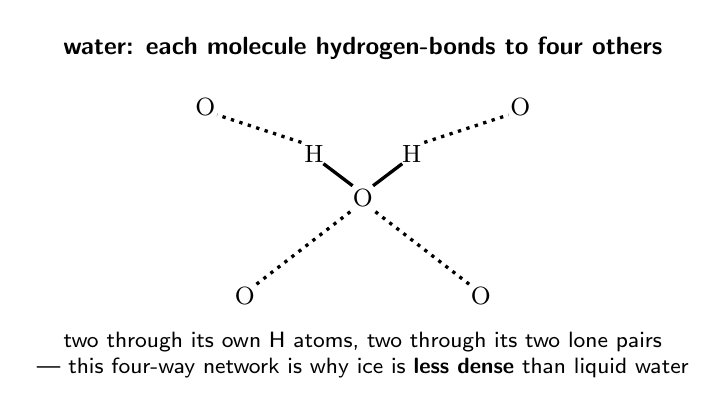
\begin{tikzpicture}[font=\sffamily\footnotesize]
  % central water molecule with four H-bonds
  \node[font=\sffamily\small\bfseries] at (0,3.3) {water: each molecule
    hydrogen-bonds to four others};
  \node[font=\small] at (0,1.4) {O};
  \node[font=\small] at (-0.62,1.95) {H};
  \node[font=\small] at (0.62,1.95) {H};
  \draw[very thick] (-0.13,1.55) -- (-0.5,1.83);
  \draw[very thick] (0.13,1.55) -- (0.5,1.83);
  % four neighbours
  \node[font=\small] at (-2.0,2.55) {O};
  \node[font=\small] at (2.0,2.55) {O};
  \node[font=\small] at (-1.5,0.15) {O};
  \node[font=\small] at (1.5,0.15) {O};
  \draw[dotted,very thick] (-0.78,2.1) -- (-1.85,2.45);
  \draw[dotted,very thick] (0.78,2.1) -- (1.85,2.45);
  \draw[dotted,very thick] (-0.16,1.22) -- (-1.35,0.3);
  \draw[dotted,very thick] (0.16,1.22) -- (1.35,0.3);
  \node[align=center] at (0,-0.6)
    {two through its own H atoms, two through its two lone pairs\\
     --- this four-way network is why ice is \textbf{less dense} than
     liquid water};
\end{tikzpicture}
\end{center}

The clearest evidence that hydrogen bonding is real is a graph. Boiling
points normally rise down a group as clouds grow. In three groups the
first member breaks the rule badly.

\begin{center}
\begin{tikzpicture}
\begin{axis}[
  width=11.5cm, height=6.6cm,
  xlabel={period of the central atom}, ylabel={boiling point
    (\si{\celsius})},
  xmin=1.6, xmax=5.4, ymin=-190, ymax=130,
  xtick={2,3,4,5}, ytick={-150,-100,-50,0,50,100},
  grid=major, grid style={apcgray!25},
  % north east, not south east: the data all sinks toward the lower
  % right, and a south-east legend sat directly on top of all three
  % lines.  Only the top-right corner is genuinely empty.
  legend pos=north east, legend style={font=\footnotesize,
    cells={anchor=west}},
  label style={font=\footnotesize}, tick label style={font=\footnotesize},
]
% group 16: H2O H2S H2Se H2Te
\addplot[seriesA, mark=*, mark size=1.6pt]
  coordinates {(2,100) (3,-60) (4,-41) (5,-2)};
\addlegendentry{group 16 (\ce{H2O}\ldots)}
% group 17: HF HCl HBr HI
\addplot[seriesB, mark=square*, mark size=1.6pt]
  coordinates {(2,20) (3,-85) (4,-67) (5,-35)};
\addlegendentry{group 17 (\ce{HF}\ldots)}
% group 14: CH4 SiH4 GeH4 SnH4
\addplot[seriesC, mark=triangle*, mark size=2pt]
  coordinates {(2,-164) (3,-112) (4,-88) (5,-52)};
\addlegendentry{group 14 (\ce{CH4}\ldots) --- no anomaly}
\end{axis}
\end{tikzpicture}
\end{center}

\begin{apctrap}
\textbf{Read the group-14 line.} It rises smoothly with no kink, because
carbon is not N, O or F and \ce{CH4} cannot hydrogen-bond. It is the
control that proves the other two lines are showing something real ---
and it is the line students forget to mention when a question asks for
evidence.
\end{apctrap}

\begin{workedexample}[I do: reading the anomaly]
\textbf{Why does \ce{H2O} boil at \SI{100}{\celsius} when \ce{H2S},
which is heavier, boils at \SI{-60}{\celsius}?}

\textbf{Start with what the trend predicts.} \ce{H2S} has more electrons
than \ce{H2O}, so on dispersion grounds alone it should boil
\emph{higher}. Extrapolating the \ce{H2S}--\ce{H2Se}--\ce{H2Te} line
backwards predicts about \SI{-80}{\celsius} for water.

\textbf{Water beats that prediction by roughly \SI{180}{\celsius}.} That
gap is the size of the effect being explained --- quote it, because it
shows the effect is not a minor correction.

\textbf{The cause.} Oxygen is small and highly electronegative, so the
\ce{O-H} bond is strongly polarized and the hydrogen is left with very
little electron density --- close to a bare proton. It can approach a
lone pair on a neighbouring oxygen far more closely than any ordinary
dipole--dipole contact allows, and the attraction is correspondingly
strong. Sulfur is larger and much less electronegative, so \ce{H2S} gets
only ordinary dipole--dipole forces.

\textbf{And the consequence you live inside:} without hydrogen bonding,
water would boil near \SI{-80}{\celsius} and no ocean would exist.
\end{workedexample}

\begin{yourturn}[YOUR TURN 3 --- four questions]
\begin{enumerate}[leftmargin=*,itemsep=0.5em]
  \item Can \ce{HCl} hydrogen-bond? Explain. \workspace[1.6cm]
  \item \ce{CH3OCH3} and \ce{CH3CH2OH} have the same formula
        \ce{C2H6O}. Which boils higher, and why? \workspace[1.8cm]
  \item Why does the group-14 line show no anomaly?
        \workspace[1.6cm]
  \item Why does ice float? \workspace[1.6cm]
\end{enumerate}
\selfcheck{(a) no --- Cl is not N, O or F \quad (b) ethanol, it has
\ce{-OH} \quad (c) carbon is not N, O or F \quad (d) the H-bond network
holds molecules further apart}
\keyonly{\begin{apcanswer}(a) \textbf{No.} Hydrogen bonding requires H
bonded directly to N, O or F. Chlorine is electronegative but too large,
so its electron density is too spread out to leave the hydrogen
sufficiently bare. \ce{HCl} has ordinary dipole--dipole forces only.
(b) \textbf{Ethanol}, \ce{CH3CH2OH} (\SI{78}{\celsius}) versus dimethyl
ether (\SI{-24}{\celsius}). Ethanol has its H on the oxygen and can
hydrogen-bond; in the ether both hydrogens sit on carbon, so it manages
only dipole--dipole. Same formula, same electrons --- the whole
difference is hydrogen bonding. (c) Because carbon is \textbf{not N, O or
F}, so no member of the series can hydrogen-bond, and the boiling points
rise smoothly with electron count as dispersion alone predicts. (d)
Because each water molecule hydrogen-bonds to \textbf{four} others in a
fixed tetrahedral arrangement, and that open framework holds the
molecules \emph{further apart} than the jostling of the liquid does. Ice
is therefore less dense than liquid water and floats --- almost unique
among substances.\end{apcanswer}}
\end{yourturn}

% =====================================================================
\section*{\sffamily Ladder 4 \textbullet\ Ranking boiling points}
\zsec{10.1--10.2}

The chapter's most-asked question type. There is a fixed order of
priority, and following it beats intuition every time.

\begin{center}
\begin{tikzpicture}[font=\sffamily\footnotesize]
  \foreach \y/\n/\t/\r in {%
      3.2/1/{ionic or network solid}/{hundreds of \si{\kilo\joule\per\mole}},
      2.4/2/{hydrogen bonding}/{$\sim$\SI{20}{\kilo\joule\per\mole}},
      1.6/3/{dipole--dipole}/{$\sim$5--\SI{25}{\kilo\joule\per\mole}},
      0.8/4/{dispersion --- but size can beat all of the above}/{varies hugely}} {
    \node[anchor=west,font=\sffamily\bfseries] at (0,\y) {\n.};
    \node[anchor=west] at (0.55,\y) {\t};
    \node[anchor=east,font=\sffamily\footnotesize\itshape] at (11.6,\y) {\r};}
  \draw[-{Stealth[length=3mm]},very thick] (-0.35,3.45) -- (-0.35,0.55);
  \node[rotate=90,font=\sffamily\footnotesize] at (-0.75,2.0) {check in
    this order};
\end{tikzpicture}
\end{center}

\begin{apctrap}
Rule 4 is the one that catches people. Dispersion is weakest
\emph{per interaction}, but it scales without limit --- so \ce{I2}
(dispersion only) boils at \SI{184}{\celsius} while \ce{H2O} (hydrogen
bonded) boils at \SI{100}{\celsius}. Compare like with like: rank by
force type only when the molecules are of \emph{similar size}, and by
size when the force types match.
\end{apctrap}

\begin{workedexample}[I do: rank four substances]
\textbf{Rank by increasing boiling point: \ce{CH4}, \ce{CH3OH},
\ce{CH3F}, \ce{NaCl}.}

\textbf{Classify each first --- never compare before classifying.}
\begin{center}
\begin{tabular}{@{}llll@{}}
\toprule
& \textbf{particles} & \textbf{strongest force} & \textbf{electrons} \\
\midrule
\ce{CH4}   & molecules & dispersion only   & 10 \\
\ce{CH3F}  & molecules & dipole--dipole    & 18 \\
\ce{CH3OH} & molecules & hydrogen bonding  & 18 \\
\ce{NaCl}  & ions      & ionic (not an IMF at all) & --- \\
\bottomrule
\end{tabular}
\end{center}

\textbf{Now apply the order.} \ce{NaCl} is ionic, so it sits far above
every molecular substance --- it is not a stronger intermolecular force,
it is a different category. Among the three molecules, \ce{CH3OH}
hydrogen-bonds and so beats \ce{CH3F}, which is polar and so beats
\ce{CH4}, which has dispersion only.

\textbf{The three molecules are close enough in size} (10 and 18
electrons) that the force type decides, so rule 4 does not overturn
anything here.
\[ \ce{CH4} \;<\; \ce{CH3F} \;<\; \ce{CH3OH} \;<\; \ce{NaCl} \]
Actual values: \SI{-164}{\celsius}, \SI{-78}{\celsius},
\SI{65}{\celsius}, \SI{1413}{\celsius} --- note the jump of over
\SI{1300}{\celsius} to the ionic solid.
\end{workedexample}

\begin{yourturn}[YOUR TURN 4 --- four questions]
\begin{enumerate}[leftmargin=*,itemsep=0.5em]
  \item Rank by increasing boiling point: \ce{Ne}, \ce{HF}, \ce{Xe}.
        \workspace[1.6cm]
  \item Rank by increasing boiling point: \ce{C2H6}, \ce{CH3OH},
        \ce{CH3Cl}. \workspace[1.6cm]
  \item Which boils higher, \ce{H2O} or \ce{I2}? What does the answer
        show? \workspace[1.8cm]
  \item Why does \ce{MgO} melt so much higher than \ce{NaCl}?
        \workspace[1.8cm]
\end{enumerate}
\selfcheck{(a) Ne $<$ Xe $<$ HF \quad (b) \ce{C2H6} $<$ \ce{CH3Cl} $<$
\ce{CH3OH} \quad (c) \ce{I2} --- size can beat force type \quad (d)
$2+/2-$ charges instead of $1+/1-$}
\keyonly{\begin{apcanswer}(a) \textbf{\ce{Ne} $<$ \ce{Xe} $<$ \ce{HF}}
(\SI{-246}{}, \SI{-108}{}, \SI{20}{\celsius}). Both noble gases have
dispersion only, so \ce{Xe} wins on size; \ce{HF} hydrogen-bonds and
beats both. (b) \textbf{\ce{C2H6} $<$ \ce{CH3Cl} $<$ \ce{CH3OH}}
(\SI{-89}{}, \SI{-24}{}, \SI{65}{\celsius}) --- dispersion only, then
dipole--dipole, then hydrogen bonding, with sizes close enough that force
type decides. (c) \textbf{\ce{I2}} (\SI{184}{\celsius}) boils higher than
\ce{H2O} (\SI{100}{\celsius}), even though water hydrogen-bonds and
\ce{I2} has dispersion only. It shows that \textbf{force type alone never
settles a ranking} --- \ce{I2} has 106 electrons to water's 10, and
enough dispersion beats hydrogen bonding. (d) Lattice energy scales with
the product of the ion charges. \ce{NaCl} pairs $1+$ with $1-$ (product
1); \ce{MgO} pairs $2+$ with $2-$ (product 4), so its attractions are
about four times stronger --- \SI{2852}{\celsius} against
\SI{801}{\celsius}.\end{apcanswer}}
\end{yourturn}

% =====================================================================
\section*{\sffamily Ladder 5 \textbullet\ Surface tension, viscosity,
capillary action}
\zsec{10.2}

Three liquid properties, one explanation: all three measure how strongly
the molecules hold each other.

\begin{center}
\begin{tikzpicture}[font=\sffamily\footnotesize]
  % water in glass: concave meniscus, rises
  \node[font=\sffamily\small\bfseries] at (1.2,3.5) {water in glass};
  \draw[very thick] (0.45,0.2) -- (0.45,3.0);
  \draw[very thick] (1.95,0.2) -- (1.95,3.0);
  \draw[very thick] (0.45,0.2) -- (1.95,0.2);
  \fill[apcgray!30] (0.45,0.2) rectangle (1.95,2.0);
  \fill[white] (1.2,2.34) ellipse (0.75 and 0.34);
  \draw[very thick] (0.45,2.0) .. controls (0.85,2.32) and (1.55,2.32)
    .. (1.95,2.0);
  \node[align=center] at (1.2,-0.5)
    {\textbf{concave} --- adhesion to glass\\beats cohesion; water
     \textbf{rises}};

  % mercury: convex, depressed
  \begin{scope}[xshift=4.2cm]
    \node[font=\sffamily\small\bfseries] at (1.2,3.5) {mercury in glass};
    \draw[very thick] (0.45,0.2) -- (0.45,3.0);
    \draw[very thick] (1.95,0.2) -- (1.95,3.0);
    \draw[very thick] (0.45,0.2) -- (1.95,0.2);
    \fill[apcgray!55] (0.45,0.2) rectangle (1.95,1.85);
    \fill[apcgray!55] (1.2,1.85) ellipse (0.75 and 0.32);
    \draw[very thick] (0.45,1.85) .. controls (0.85,2.2) and (1.55,2.2)
      .. (1.95,1.85);
    \node[align=center] at (1.2,-0.5)
      {\textbf{convex} --- cohesion beats\\adhesion; mercury
       \textbf{sinks}};
  \end{scope}

  % droplet / surface tension
  \begin{scope}[xshift=8.6cm]
    \node[font=\sffamily\small\bfseries] at (1.5,3.5) {surface tension};
    \fill[apcgray!30] (1.5,1.75) circle (0.85);
    \foreach \a in {0,45,90,135,180,225,270,315} {
      \draw[-{Stealth[length=2mm]},thick]
        ([shift={(1.5,1.75)}]\a:0.62) -- ([shift={(1.5,1.75)}]\a:0.2);}
    \fill (1.5,1.75) circle (0.07);
    \node[align=center] at (1.5,-0.5)
      {a surface molecule is pulled\\only \emph{inward} --- the drop
       pulls\\itself into a sphere};
  \end{scope}
\end{tikzpicture}
\end{center}

\begin{workedexample}[I do: three properties, one cause]
\textbf{Surface tension} is the energy needed to increase a liquid's
surface area. A molecule in the bulk is pulled equally in all
directions; a molecule at the surface has neighbours only below and to
the sides, so the net pull is inward. The liquid minimizes its surface,
which for a free drop means a sphere. Water's surface tension is high
because hydrogen bonding is strong --- high enough to support a paperclip
or a water strider.

\textbf{Viscosity} is resistance to flow. It rises with stronger
intermolecular forces, and also with molecular length, because long
molecules tangle. Glycerol, \ce{C3H5(OH)3}, carries \emph{three} \ce{-OH}
groups per molecule and pours like syrup; propane, of similar size but
with no \ce{-OH} at all, is a gas.

\textbf{Capillary action} is the competition between two forces:
\textbf{cohesion} (liquid to itself) and \textbf{adhesion} (liquid to
the container). In a glass tube water adheres to the \ce{-OH} groups on
the glass surface more strongly than it coheres to itself, so it climbs
the walls and its meniscus curves \emph{up} at the edges --- concave.
Mercury is a metal held by strong metallic bonding, coheres far more
strongly than it adheres to glass, and does the reverse: it is pushed
down and its meniscus is convex.

\textbf{The unifying statement:} strong intermolecular forces give high
surface tension and high viscosity; whether a liquid rises or sinks in a
tube depends on cohesion \emph{versus} adhesion, not on either alone.
\end{workedexample}

\begin{yourturn}[YOUR TURN 5 --- four questions]
\begin{enumerate}[leftmargin=*,itemsep=0.5em]
  \item Which has the higher surface tension, water or hexane? Why?
        \workspace[1.6cm]
  \item Why is glycerol far more viscous than ethanol?
        \workspace[1.6cm]
  \item Why does water's meniscus curve up but mercury's curve down?
        \workspace[1.8cm]
  \item What happens to a liquid's viscosity as it is heated? Explain.
        \workspace[1.8cm]
\end{enumerate}
\selfcheck{(a) water --- hydrogen bonding \quad (b) three \ce{-OH}
groups \quad (c) adhesion vs cohesion \quad (d) it falls}
\keyonly{\begin{apcanswer}(a) \textbf{Water.} It hydrogen-bonds, whereas
hexane is nonpolar with dispersion forces only, so far more energy is
needed to bring a water molecule to the surface. (b) Glycerol has
\textbf{three \ce{-OH} groups} per molecule to ethanol's one, so each
molecule hydrogen-bonds to many neighbours at once and the network
resists flow strongly. (c) Water \textbf{adheres} to the polar \ce{-OH}
groups on glass more strongly than it \textbf{coheres} to itself, so it
climbs the walls (concave). Mercury's metallic bonding makes cohesion
much stronger than its adhesion to glass, so it pulls away from the
walls (convex). (d) It \textbf{falls}. Heating gives molecules more
kinetic energy, so they overcome the intermolecular attractions holding
them in place more easily and the liquid flows more freely --- which is
why warm syrup pours and cold syrup does not.\end{apcanswer}}
\end{yourturn}

% =====================================================================
\section*{\sffamily Ladder 6 \textbullet\ Metallic solids and the
electron sea}
\zsec{10.3--10.4}

A metal is a lattice of cations sitting in a sea of electrons that
belong to no particular atom. Every metallic property follows from
those mobile electrons.

\begin{center}
\begin{tikzpicture}[font=\sffamily\footnotesize]
  \node[font=\sffamily\small\bfseries] at (2.2,3.4) {the electron-sea
    model};
  \fill[apcgray!18] (0.1,0.35) rectangle (4.3,2.9);
  \foreach \x in {0.65,1.55,2.45,3.35} {
    \foreach \y in {0.85,1.65,2.45} {
      \fill[apcgray!60] (\x,\y) circle (0.23);
      \node[font=\tiny] at (\x,\y) {$+$};}}
  \foreach \x/\y in {1.1/1.25, 2.0/2.05, 2.9/1.25, 1.1/2.05, 2.0/0.6,
                     3.8/1.65, 0.3/1.65, 2.9/2.45, 3.8/0.85} {
    \fill (\x,\y) circle (0.06);}
  \node[align=center] at (2.2,-0.35)
    {fixed cations \textbullet\ delocalized electrons free to move};

  % consequences
  \node[anchor=west,align=left] at (5.0,2.45)
    {\textbf{conducts electricity} --- electrons move};
  \node[anchor=west,align=left] at (5.0,1.85)
    {\textbf{conducts heat} --- electrons carry energy};
  \node[anchor=west,align=left] at (5.0,1.25)
    {\textbf{lustrous} --- electrons re-emit light};
  \node[anchor=west,align=left] at (5.0,0.65)
    {\textbf{malleable} --- see below};
\end{tikzpicture}
\end{center}

\begin{center}
\begin{tikzpicture}[font=\sffamily\footnotesize]
  % metal deforms
  \node[font=\sffamily\small\bfseries] at (1.8,2.9) {metal under stress};
  \foreach \x in {0.4,1.2,2.0,2.8} {
    \foreach \y in {0.9,1.7} {
      \fill[apcgray!60] (\x,\y) circle (0.2);
      \node[font=\tiny] at (\x,\y) {$+$};}}
  \draw[-{Stealth[length=2.5mm]},very thick] (0.2,2.25) -- (3.0,2.25);
  \node[align=center] at (1.8,0.1)
    {layers slide, the electron sea\\follows --- it \textbf{bends}};

  % Ionic: drawn in the SHIFTED state, so the figure actually shows the
  % like-on-like collision its caption describes.  The previous version
  % drew an undisplaced lattice and asserted the shift in words only.
  \begin{scope}[xshift=6.2cm]
    \node[font=\sffamily\small\bfseries] at (2.0,2.9) {ionic under
      stress};
    % bottom row, alternating, in its original position
    \foreach \x/\q in {0.4/{$+$}, 1.2/{$-$}, 2.0/{$+$}, 2.8/{$-$}} {
      \fill[apcgray!60] (\x,0.9) circle (0.2);
      \node[font=\tiny] at (\x,0.9) {\q};}
    % top row, slid RIGHT by one ion width
    \foreach \x/\q in {1.2/{$-$}, 2.0/{$+$}, 2.8/{$-$}, 3.6/{$+$}} {
      \fill[apcgray!60] (\x,1.7) circle (0.2);
      \node[font=\tiny] at (\x,1.7) {\q};}
    % like now faces like: mark the repulsions
    \foreach \x in {1.2,2.0,2.8} {
      \draw[{Stealth[length=2mm]}-{Stealth[length=2mm]},thick]
        (\x,1.47) -- (\x,1.13);}
    \draw[-{Stealth[length=2.5mm]},very thick] (0.4,2.25) -- (3.2,2.25);
    \node[align=center] at (2.0,0.1)
      {the shift puts like on like\\--- it \textbf{shatters}};
  \end{scope}
\end{tikzpicture}
\end{center}

\begin{workedexample}[I do: why metals bend and salts shatter]
\textbf{Hit a copper sheet and it dents. Hit a salt crystal and it
splits.} Both are held by strong electrostatic forces, so why the
opposite behaviour?

\textbf{In the metal, the bonding is non-directional.} The cations are
all positive and the electron sea surrounds all of them equally. Slide
one layer of cations past another and every cation is still in the same
sea, still attracted in every direction. The bonding is undisturbed, so
the metal simply takes the new shape --- it is \textbf{malleable} and
\textbf{ductile}.

\textbf{In the ionic solid, the bonding is exactly directional.} Each
cation is surrounded by anions and vice versa. Slide one layer by a
single ion's width and now cations face cations, anions face anions. The
attraction becomes a \emph{repulsion} along the whole plane, and the
crystal flies apart --- it is \textbf{brittle}.

\textbf{The conductivity test tells them apart too.} A metal conducts as
a solid, because its electrons are already mobile. An ionic solid does
\emph{not} conduct as a solid --- its ions are locked in the lattice ---
but conducts well once molten or dissolved, because then the ions can
move. If a substance conducts when solid, it is a metal (or graphite);
if only when molten, it is ionic.
\end{workedexample}

\begin{yourturn}[YOUR TURN 6 --- four questions]
\begin{enumerate}[leftmargin=*,itemsep=0.5em]
  \item Why does a metal conduct electricity as a solid but \ce{NaCl}
        does not? \workspace[1.8cm]
  \item Why is an ionic crystal brittle? \workspace[1.8cm]
  \item An unknown solid conducts when molten but not when solid. What
        type is it? \workspace[1.6cm]
  \item Why do metals conduct heat well? \workspace[1.6cm]
\end{enumerate}
\selfcheck{(a) delocalized electrons vs locked ions \quad (b) a shift
puts like charges together \quad (c) ionic \quad (d) mobile electrons
carry the energy}
\keyonly{\begin{apcanswer}(a) A metal's valence electrons are
\textbf{delocalized} and free to move through the whole lattice, so a
current flows. In solid \ce{NaCl} the charge carriers are \textbf{ions},
and they are locked in fixed lattice positions, so no charge can move.
(b) Because the lattice alternates cation and anion. Displacing one
layer by a single ion's width brings \textbf{like charges face to face},
turning attraction into repulsion along the whole plane and splitting the
crystal. (c) \textbf{Ionic.} Conducting only when molten means the
carriers are ions that must be freed from the lattice first --- a metal
would conduct in both states, and a molecular solid in neither. (d)
Their \textbf{mobile electrons} carry kinetic energy rapidly through the
solid, rather than energy having to pass slowly from one vibrating
particle to the next as in an insulator.\end{apcanswer}}
\end{yourturn}

% =====================================================================
\section*{\sffamily Ladder 7 \textbullet\ Unit cells and counting atoms}
\zsec{10.4}

A crystal is one small pattern repeated. The \textbf{unit cell} is that
pattern, and the trick is that atoms on the boundary are shared with
neighbouring cells.

\begin{center}
\begin{tikzpicture}[font=\sffamily\footnotesize, scale=0.95]
  \foreach \i/\nm/\cnt/\cn/\pk in {%
      0/{simple cubic}/{1 atom}/{6}/{52\%},
      4.6/{body-centred cubic}/{2 atoms}/{8}/{68\%},
      9.2/{face-centred cubic}/{4 atoms}/{12}/{74\%}} {
    \begin{scope}[xshift=\i cm]
      \node[font=\sffamily\small\bfseries] at (1.35,3.55) {\nm};
      % cube outline (oblique projection)
      \draw[thick] (0.3,0.3) rectangle (2.1,2.1);
      \draw[thick] (0.9,0.9) rectangle (2.7,2.7);
      \draw[thick] (0.3,0.3) -- (0.9,0.9);
      \draw[thick] (2.1,0.3) -- (2.7,0.9);
      \draw[thick] (0.3,2.1) -- (0.9,2.7);
      \draw[thick] (2.1,2.1) -- (2.7,2.7);
      \node[align=center] at (1.5,-0.35)
        {\cnt\ per cell\\CN \cn\ \textbullet\ \pk\ full};
    \end{scope}}
  % corners on all three
  \foreach \i in {0,4.6,9.2} {
    \begin{scope}[xshift=\i cm]
      \foreach \p in {(0.3,0.3),(2.1,0.3),(0.3,2.1),(2.1,2.1),
                      (0.9,0.9),(2.7,0.9),(0.9,2.7),(2.7,2.7)} {
        \fill[apcgray!60] \p circle (0.19);}
    \end{scope}}
  % bcc body centre
  \begin{scope}[xshift=4.6cm]
    \fill[apcgray!30] (1.5,1.5) circle (0.24);
    \draw[thick] (1.5,1.5) circle (0.24);
  \end{scope}
  % fcc face centres
  \begin{scope}[xshift=9.2cm]
    \foreach \p in {(1.2,1.2),(1.8,1.8),(0.6,1.5),(2.4,1.5),
                    (1.5,0.6),(1.5,2.4)} {
      \fill[apcgray!30] \p circle (0.22);
      \draw[thick] \p circle (0.22);}
  \end{scope}
\end{tikzpicture}
\end{center}

\begin{center}
\begin{tikzpicture}[font=\sffamily\footnotesize]
  \node[font=\sffamily\small\bfseries] at (5.2,1.9) {how much of an atom
    belongs to \emph{this} cell};
  \foreach \x/\pos/\frac in {0.4/{corner}/{$1/8$}, 3.0/{edge}/{$1/4$},
                             5.6/{face}/{$1/2$}, 8.2/{body}/{$1$}} {
    \node[anchor=west,font=\sffamily\bfseries] at (\x,1.2) {\pos};
    \node[anchor=west] at (\x,0.7) {\frac};}
  \draw[apcgray] (0.2,0.35) -- (10.2,0.35);
  \node[font=\sffamily\footnotesize,anchor=west] at (0.4,-0.05)
    {shared between 8 cells, 4 cells, 2 cells, and nobody};
\end{tikzpicture}
\end{center}

\begin{workedexample}[I do: count the atoms, then get the density]
\textbf{Copper is face-centred cubic with a cell edge of
\SI{361.5}{\pico\metre}. Find its density.}

\textbf{Step 1 --- count the atoms in one cell.} Eight corners, each
worth $1/8$, and six faces, each worth $1/2$:
\[ 8 \times \tfrac{1}{8} \;+\; 6 \times \tfrac{1}{2}
   \;=\; 1 + 3 \;=\; \mathbf{4 \text{ atoms}} \]

\textbf{Step 2 --- mass of one cell.}
\[ m = \frac{4 \times \SI{63.55}{\gram\per\mole}}
            {\SI{6.022e23}{\per\mole}}
     = \SI{4.221e-22}{\gram} \]

\textbf{Step 3 --- volume of one cell.} Convert the edge to centimetres
first: \SI{361.5}{\pico\metre} $= \SI{3.615e-8}{\centi\metre}$.
\[ V = (\SI{3.615e-8}{\centi\metre})^{3}
     = \SI{4.724e-23}{\centi\metre\cubed} \]

\textbf{Step 4 --- divide.}
\[ d = \frac{\SI{4.221e-22}{\gram}}{\SI{4.724e-23}{\centi\metre\cubed}}
     = \SI{8.94}{\gram\per\centi\metre\cubed} \]

\textbf{Check it against reality:} copper's measured density is
\SI{8.96}{\gram\per\centi\metre\cubed}. Agreement to three figures from
nothing but a cell edge and a counting rule --- which is how we know the
model is right.

\textbf{The step everyone drops:} converting picometres to centimetres
\emph{before} cubing. Cube first and the answer is wrong by $10^{30}$.
\end{workedexample}

\begin{yourturn}[YOUR TURN 7 --- four questions]
\begin{enumerate}[leftmargin=*,itemsep=0.5em]
  \item How many atoms are in a body-centred cubic unit cell? Show the
        count. \workspace[1.6cm]
  \item How many are in a simple cubic cell? \workspace[1.4cm]
  \item Which packs most efficiently, and what fraction of space is
        empty in it? \workspace[1.6cm]
  \item A cell has atoms at all 8 corners and 1 in the centre of each of
        2 opposite faces. How many atoms per cell?
        \workspace[1.6cm]
\end{enumerate}
\selfcheck{(a) 2 \quad (b) 1 \quad (c) fcc/hcp, 26\% empty \quad (d) 2}
\keyonly{\begin{apcanswer}(a) $8 \times \frac{1}{8} + 1 = \mathbf{2}$ ---
eight corner eighths make one atom, plus the whole atom at the body
centre, which is shared with nobody. (b) $8 \times \frac{1}{8} =
\mathbf{1}$. (c) \textbf{Face-centred cubic} (cubic closest packed) and
\textbf{hexagonal closest packed} tie at \textbf{74\%} filled, so
\textbf{26\%} is empty. Both achieve coordination number 12, the maximum
for equal spheres. (d) $8 \times \frac{1}{8} + 2 \times \frac{1}{2} =
1 + 1 = \mathbf{2}$ --- each face-centre atom is shared between two
cells, whether or not the other four faces have one.\end{apcanswer}}
\end{yourturn}

% =====================================================================
\section*{\sffamily Ladder 8 \textbullet\ Alloys}
\zsec{10.4}

An alloy is a metal mixed with something else while molten. There are
two ways the guest can sit in the host lattice, and they have different
consequences.

\begin{center}
\begin{tikzpicture}[font=\sffamily\footnotesize]
  % substitutional
  \node[font=\sffamily\small\bfseries] at (2.0,3.35) {substitutional};
  \foreach \x in {0.5,1.3,2.1,2.9} {
    \foreach \y in {0.7,1.5,2.3} {
      \fill[apcgray!55] (\x,\y) circle (0.24);}}
  \fill[apcgray!15] (1.3,1.5) circle (0.24);
  \draw[thick] (1.3,1.5) circle (0.24);
  \fill[apcgray!15] (2.9,2.3) circle (0.24);
  \draw[thick] (2.9,2.3) circle (0.24);
  \node[align=center] at (1.7,-0.15)
    {similar-sized atoms \textbf{replace}\\host atoms in the lattice\\
     \emph{brass} (\ce{Cu}$+$\ce{Zn}), \emph{sterling silver}};

  % interstitial
  \begin{scope}[xshift=7.0cm]
    \node[font=\sffamily\small\bfseries] at (2.0,3.35) {interstitial};
    \foreach \x in {0.5,1.3,2.1,2.9} {
      \foreach \y in {0.7,1.5,2.3} {
        \fill[apcgray!55] (\x,\y) circle (0.24);}}
    \foreach \p in {(0.9,1.1),(1.7,1.9),(2.5,1.1)} {
      \fill \p circle (0.1);}
    \node[align=center] at (1.7,-0.15)
      {much smaller atoms sit in the\\\textbf{holes} between host
       atoms\\\emph{steel} (\ce{Fe}$+$\ce{C})};
  \end{scope}
\end{tikzpicture}
\end{center}

\begin{workedexample}[I do: why a trace of carbon transforms iron]
\textbf{Pure iron is soft enough to bend by hand at the right thickness.
Steel --- iron with under 2\% carbon --- builds bridges. Two percent of
anything should not do that.}

\textbf{Recall why pure metals are soft.} They deform because layers of
cations \emph{slide} over one another without disturbing the electron
sea. Malleability is that sliding.

\textbf{Now block the sliding.} Carbon atoms are far smaller than iron
atoms, so they fit into the holes between them --- an
\textbf{interstitial} alloy. They sit directly in the slip planes, and a
layer trying to slide has to climb over them. The sliding stops, and the
metal becomes hard and strong instead of soft and bendable.

\textbf{Substitutional alloys work differently.} In brass, zinc atoms
are close enough in size to copper (\SI{134}{} against
\SI{128}{\pico\metre}) to take copper's place in the lattice outright.
They still disrupt its regularity, and so still harden the metal, but far
less dramatically --- the alloy keeps much of the host's character, and
brass stays workable enough to be chosen for its colour and corrosion
resistance as much as for its strength.

\textbf{The size test decides which you have:} similar-sized guest
$\Rightarrow$ substitutional; much smaller guest $\Rightarrow$
interstitial.
\end{workedexample}

\begin{yourturn}[YOUR TURN 8 --- four questions]
\begin{enumerate}[leftmargin=*,itemsep=0.5em]
  \item Classify brass (\ce{Cu} with \ce{Zn}) and say why.
        \workspace[1.6cm]
  \item Classify steel and say why. \workspace[1.6cm]
  \item Why is steel harder than pure iron? \workspace[1.8cm]
  \item Would a guest atom twice the host's diameter form an
        interstitial alloy? Explain. \workspace[1.8cm]
\end{enumerate}
\selfcheck{(a) substitutional --- similar radii \quad (b) interstitial
--- C is much smaller \quad (c) interstitials block layer sliding \quad
(d) no --- far too large for the holes}
\keyonly{\begin{apcanswer}(a) \textbf{Substitutional.} Copper and zinc
have very similar atomic radii (\SI{128}{} and \SI{134}{\pico\metre}),
so zinc atoms simply take copper's places in the lattice. (b)
\textbf{Interstitial.} Carbon is far smaller than iron, so it occupies
the holes between iron atoms rather than replacing them. (c) Because the
carbon atoms sit in the \textbf{slip planes} and physically obstruct
layers of iron cations from sliding past one another. Malleability
\emph{is} that sliding, so blocking it converts a soft metal into a hard
one. (d) \textbf{No.} Interstitial sites are the small gaps left between
close-packed host atoms; an atom larger than the host could not possibly
fit into one. Such an atom could not form a substitutional alloy either
--- it would distort the lattice too severely --- so the two metals would
simply not be miscible in the solid.\end{apcanswer}}
\end{yourturn}

% =====================================================================
\section*{\sffamily Ladder 9 \textbullet\ Network covalent and molecular
solids}
\zsec{10.5--10.6}

The largest gap in properties anywhere in chemistry sits between these
two, and both are made only of nonmetals.

\begin{center}
\begin{tikzpicture}[font=\sffamily\footnotesize]
  % diamond
  \node[font=\sffamily\small\bfseries] at (2.0,3.5) {diamond};
  \foreach \x/\y in {0.6/0.6, 2.0/0.6, 3.4/0.6, 1.3/1.7, 2.7/1.7,
                     0.6/2.8, 2.0/2.8, 3.4/2.8} {
    \fill[apcgray!60] (\x,\y) circle (0.17);}
  \draw[thick] (0.6,0.6) -- (1.3,1.7) -- (2.0,0.6);
  \draw[thick] (2.0,0.6) -- (2.7,1.7) -- (3.4,0.6);
  \draw[thick] (1.3,1.7) -- (0.6,2.8);
  \draw[thick] (1.3,1.7) -- (2.0,2.8);
  \draw[thick] (2.7,1.7) -- (2.0,2.8);
  \draw[thick] (2.7,1.7) -- (3.4,2.8);
  \node[align=center] at (2.0,-0.35)
    {every C is $sp^{3}$, bonded to \textbf{four}\\
     one giant molecule \textbullet\ mp \SI{3550}{\celsius}\\
     hardest known \textbullet\ insulator};

  % graphite
  \begin{scope}[xshift=6.8cm]
    \node[font=\sffamily\small\bfseries] at (2.2,3.5) {graphite};
    \foreach \yy in {0.7,1.75,2.8} {
      \foreach \xx in {0.5,1.1,1.7,2.3,2.9,3.5} {
        \fill[apcgray!60] (\xx,\yy) circle (0.13);}
      \draw[thick] (0.5,\yy) -- (3.5,\yy);}
    \foreach \yy in {1.05,2.1} {
      \foreach \xx in {0.8,1.7,2.6,3.5} {
        \draw[dotted,thick] (\xx,\yy) -- (\xx,\yy+0.35);}}
    \node[align=center] at (2.0,-0.35)
      {sheets seen \textbf{edge-on}; each C is $sp^{2}$\\
       strong sheets, \textbf{weak} LDF between\\
       conducts in-plane \textbullet\ slippery};
  \end{scope}
\end{tikzpicture}
\end{center}

\begin{apctrap}
\textbf{Graphite is the exception that a question will test.} It is a
network covalent solid that \emph{conducts}, because each carbon uses
only three of its four valence electrons for $\sigma$ bonds and the
fourth is delocalized across the sheet. It is also soft, because the
sheets are held to each other only by dispersion forces and slide freely
--- which is why a pencil writes. Same element as diamond, opposite
properties, and the reason is the bonding pattern, not the element.
\end{apctrap}

\begin{workedexample}[I do: classify a solid from its properties]
A table for the four solid types, and the way a question will hand them
to you --- as properties, not as names.

\begin{center}
\renewcommand{\arraystretch}{1.25}
\begin{tabular}{@{}lllll@{}}
\toprule
\textbf{type} & \textbf{particles} & \textbf{force} &
  \textbf{melting pt} & \textbf{conducts?} \\
\midrule
ionic     & ions          & ionic attraction & high      &
  molten/aq only \\
metallic  & cations $+$ e$^-$ & metallic bond & varies wildly &
  always \\
network   & atoms         & covalent bonds   & very high &
  no (graphite yes) \\
molecular & molecules     & IMF              & low       & no \\
\bottomrule
\end{tabular}
\end{center}

\textbf{Worked case: a solid melts at \SI{-57}{\celsius}, does not
conduct in any state, and is soft.}

Very low melting point rules out ionic, network and most metals at once.
No conduction in any state rules out metallic (which conducts solid) and
ionic (which conducts molten). Softness confirms it. This is a
\textbf{molecular solid}: the particles are whole molecules, and melting
only has to overcome \emph{intermolecular forces} --- no bond breaks at
all.

\textbf{The diagnostic question is always the same:} what has to break
for this to melt? A molecular solid breaks weak forces \emph{between}
molecules; a network solid breaks covalent bonds \emph{themselves}. That
single difference spans \SI{3600}{\celsius}.
\end{workedexample}

\begin{yourturn}[YOUR TURN 9 --- four questions]
\begin{enumerate}[leftmargin=*,itemsep=0.5em]
  \item \ce{SiO2} melts at \SI{1610}{\celsius}; \ce{CO2} melts at
        \SI{-57}{\celsius} under pressure, and at \SI{1}{atm} does not
        melt at all but sublimes at \SI{-78}{\celsius}. Both are
        group-14 dioxides. Explain. \workspace[1.8cm]
  \item Why is graphite soft when diamond is the hardest substance
        known? \workspace[1.8cm]
  \item Why does graphite conduct but diamond not? \workspace[1.8cm]
  \item A solid is hard, melts above \SI{2000}{\celsius}, and does not
        conduct even when molten. Classify it. \workspace[1.6cm]
\end{enumerate}
\selfcheck{(a) \ce{SiO2} is network, \ce{CO2} molecular \quad (b) sheets
slide on weak LDF \quad (c) a delocalized fourth electron \quad (d)
network covalent}
\keyonly{\begin{apcanswer}(a) \ce{SiO2} is a \textbf{network covalent}
solid --- silicon forms four single \ce{Si-O} bonds and the whole crystal
is one molecule, so melting means breaking covalent bonds. \ce{CO2} is
\textbf{molecular}: carbon forms two double bonds and the molecule is
complete, so melting only overcomes weak dispersion forces between
separate \ce{CO2} molecules. (b) Diamond is covalently bonded in all
three dimensions, so deforming it means breaking covalent bonds. In
graphite the covalent bonding is confined to \textbf{flat sheets}, which
are held to one another only by \textbf{dispersion forces} and slide over
each other easily. (c) Each graphite carbon is $sp^{2}$ and uses three
valence electrons for $\sigma$ bonds, leaving the \textbf{fourth
delocalized} across the sheet and free to carry current. Every one of
diamond's four valence electrons is locked into a localized $\sigma$
bond, so none is mobile. (d) \textbf{Network covalent.} The very high
melting point and hardness point to covalent bonds throughout, and the
absence of conduction \emph{even when molten} rules out ionic --- molten
ionic compounds always conduct.\end{apcanswer}}
\end{yourturn}

% =====================================================================
\section*{\sffamily Ladder 10 \textbullet\ Ionic solids}
\zsec{10.7}

An ionic crystal is built so that each ion is surrounded by as many
oppositely charged neighbours as will geometrically fit --- which is
what makes lattice energies so large.

\begin{center}
\begin{tikzpicture}[font=\sffamily\footnotesize]
  % Title raised to 4.4: the top row of ions reaches y=3.9 and printed
  % straight through it at 3.65.
  \node[font=\sffamily\small\bfseries] at (2.1,4.4) {\ce{NaCl}: each ion
    has \textbf{six} nearest neighbours};
  % 3x3 grid alternating
  \foreach \i in {0,1,2} {
    \foreach \j in {0,1,2} {
      \pgfmathsetmacro{\s}{mod(\i+\j,2)}
      \ifdim\s pt>0.5pt
        \fill[apcgray!25] (0.7+\i*1.4,0.7+\j*1.4) circle (0.4);
        \node[font=\tiny] at (0.7+\i*1.4,0.7+\j*1.4) {\ce{Cl^-}};
      \else
        \fill[apcgray!65] (0.7+\i*1.4,0.7+\j*1.4) circle (0.24);
        \node[font=\tiny] at (0.7+\i*1.4,0.7+\j*1.4) {\ce{Na^+}};
      \fi}}
  % highlight the central ion's neighbours
  \draw[very thick] (2.1,2.1) -- (0.7,2.1);
  \draw[very thick] (2.1,2.1) -- (3.5,2.1);
  \draw[very thick] (2.1,2.1) -- (2.1,0.7);
  \draw[very thick] (2.1,2.1) -- (2.1,3.5);
  \node[align=left,anchor=west] at (5.0,2.9)
    {four neighbours shown in the plane};
  \node[align=left,anchor=west] at (5.0,2.3)
    {two more above and below};
  \node[align=left,anchor=west] at (5.0,1.7)
    {\textbf{coordination number 6}};
  \node[align=left,anchor=west] at (5.0,0.9)
    {\ce{Cl^-} ions form an fcc array;};
  \node[align=left,anchor=west] at (5.0,0.4)
    {\ce{Na^+} fills every octahedral hole};
\end{tikzpicture}
\end{center}

\begin{workedexample}[I do: formula from a unit cell]
\textbf{In the \ce{NaCl} unit cell, chloride ions sit at the 8 corners
and the 6 face centres, and sodium ions sit at the 12 edge midpoints and
the 1 body centre. Show the formula is \ce{NaCl}.}

\textbf{Count the chloride.} It occupies exactly the fcc positions:
\[ 8 \times \tfrac{1}{8} \;+\; 6 \times \tfrac{1}{2} \;=\; 1 + 3
   \;=\; 4 \;\ce{Cl^-} \]

\textbf{Count the sodium.} Edge atoms are shared between four cells;
the body centre belongs to this cell alone:
\[ 12 \times \tfrac{1}{4} \;+\; 1 \;=\; 3 + 1 \;=\; 4 \;\ce{Na^+} \]

\textbf{Take the ratio.} Four to four is \textbf{1:1}, giving the
empirical formula \ce{NaCl} --- exactly what charge balance demanded, now
confirmed by the geometry independently.

\textbf{Why this matters beyond the arithmetic.} There is no
``\ce{NaCl} molecule''. No sodium ion belongs to any one chloride; each
is bonded equally to six. The formula is a \emph{ratio}, which is why we
call it an empirical formula and why ionic compounds have no molecular
mass in the way \ce{CO2} does.
\end{workedexample}

\begin{yourturn}[YOUR TURN 10 --- four questions]
\begin{enumerate}[leftmargin=*,itemsep=0.5em]
  \item What is the coordination number of \ce{Na+} in \ce{NaCl}?
        \workspace[1.4cm]
  \item A cell has \ce{X} at 8 corners and \ce{Y} at the body centre.
        Give the formula. \workspace[1.6cm]
  \item Why does \ce{MgO} have a much larger lattice energy than
        \ce{NaCl}? \workspace[1.8cm]
  \item Why is it wrong to speak of an ``\ce{NaCl} molecule''?
        \workspace[1.8cm]
\end{enumerate}
\selfcheck{(a) 6 \quad (b) \ce{XY} \quad (c) $2+/2-$ charges \quad (d)
each ion binds six others equally}
\keyonly{\begin{apcanswer}(a) \textbf{6} --- four in its own plane and
one each above and below. Chloride's is also 6, so \ce{NaCl} is described
as 6:6. (b) \ce{X}: $8 \times \frac{1}{8} = 1$. \ce{Y}: $1$. Ratio 1:1,
so the formula is \textbf{\ce{XY}}. (c) Lattice energy scales with the
product of the ion charges. \ce{NaCl} pairs $1+$ with $1-$, product 1;
\ce{MgO} pairs $2+$ with $2-$, product \textbf{4}, so its attractions are
roughly four times stronger. \ce{MgO}'s ions are also slightly smaller,
which brings the centres closer and strengthens the attraction further.
(d) Because \textbf{no sodium ion is paired with any particular
chloride} --- each is surrounded by and attracted to six of them equally,
throughout a lattice that continues to the edge of the crystal.
\ce{NaCl} is an empirical \emph{ratio}, not a discrete
particle.\end{apcanswer}}
\end{yourturn}

% =====================================================================
\section*{\sffamily Ladder 11 \textbullet\ Vapour pressure and heating
curves}
\zsec{10.8}

Vapour pressure is the pressure of vapour standing above its own liquid
in a closed container once evaporation and condensation have come into
balance.

\begin{center}
\begin{tikzpicture}
\begin{axis}[
  width=11.5cm, height=6.2cm,
  xlabel={temperature (\si{\celsius})},
  ylabel={vapour pressure (torr)},
  xmin=0, xmax=110, ymin=0, ymax=850,
  xtick={0,20,40,60,80,100}, ytick={0,200,400,600,760},
  grid=major, grid style={apcgray!25},
  legend pos=north west, legend style={font=\footnotesize,
    cells={anchor=west}},
  label style={font=\footnotesize}, tick label style={font=\footnotesize},
]
% Water's domain stops at 100 -- exactly where it crosses 760, which is
% the point the graph exists to make.
\addplot[seriesA, thick, domain=0:100, samples=60]
  {4.58*exp(0.05112*x)};
\addlegendentry{water}
\addplot[seriesB, thick, domain=0:80, samples=60]
  {12.2*exp(0.05297*x)};
\addlegendentry{ethanol --- more volatile}
% The reference line starts right of the legend box; run from 0 and the
% legend sits on top of it.
\addplot[black, dashed, domain=42:110, samples=2] {760};
% Label goes at the RIGHT end -- at the left it was hidden underneath
% the legend entirely.
\node[font=\footnotesize,anchor=east] at (axis cs:109,812)
  {external pressure, 760 torr};
\end{axis}
\end{tikzpicture}
\end{center}

\begin{apcnote}[The definition of boiling, stated exactly]
A liquid boils at the temperature where its \textbf{vapour pressure
equals the external pressure}. Nothing about \SI{100}{\celsius} is
special to water --- it is the temperature at which water's vapour
pressure happens to reach \SI{760}{torr}. Lower the external pressure and
the boiling point falls with it, which is why water boils near
\SI{95}{\celsius} in Denver and why food takes longer to cook there.
\end{apcnote}

\begin{center}
\begin{tikzpicture}[font=\sffamily\footnotesize]
  \begin{axis}[
    width=12cm, height=6.4cm,
    xlabel={heat added (\si{\kilo\joule})},
    ylabel={temperature (\si{\celsius})},
    xmin=-2, xmax=60, ymin=-40, ymax=140,
    ytick={-25,0,50,100,125}, xtick={0,10,20,30,40,50},
    grid=major, grid style={apcgray!25},
    label style={font=\footnotesize},
    tick label style={font=\footnotesize},
  ]
  % ice -25 to 0 : 0.91 kJ ; fusion 6.02 ; water 7.52 ; vap 40.7 ; steam 0.90
  \addplot[seriesA, very thick] coordinates {
    (0,-25) (0.91,0) (6.93,0) (14.46,100) (55.16,100) (56.06,125)};
  % All labels horizontal and anchored WEST or EAST, never centred: a
  % centred label near x=4 extends left past the axis and gets clipped
  % (that is how "melting" printed as "nelting"), and the rotated ones
  % lay on top of the curve they were labelling.
  \node[font=\footnotesize,anchor=west] at (axis cs:1.3,-28)
    {ice warms};
  \node[font=\footnotesize,anchor=west] at (axis cs:2.0,-9)
    {melting, \SI{6.02}{\kilo\joule}};
  \node[font=\footnotesize,anchor=west] at (axis cs:15.5,55)
    {liquid warms};
  \node[font=\footnotesize,anchor=south] at (axis cs:32,103)
    {boiling, \SI{40.7}{\kilo\joule} --- the long one};
  \node[font=\footnotesize,anchor=east] at (axis cs:54,130)
    {steam warms};
  \end{axis}
\end{tikzpicture}
\end{center}

\begin{apctrap}
\textbf{Temperature does not rise on the flat parts.} All the energy
going in is breaking intermolecular forces, not speeding molecules up.
Ice water stays at \SI{0}{\celsius} until the last ice is gone --- and
that is why ice cools a drink so well.
\end{apctrap}

\begin{workedexample}[I do: heat 18.0 g of ice at $-25$\,\si{\celsius} to
steam at 125\,\si{\celsius}]
Five segments, and you must not merge them. Use $c_{\text{ice}} =
\SI{2.03}{\joule\per\gram\per\celsius}$, $c_{\text{water}} =
\SI{4.18}{}$, $c_{\text{steam}} = \SI{2.01}{}$,
$\Delta H_{\text{fus}} = \SI{6.02}{\kilo\joule\per\mole}$,
$\Delta H_{\text{vap}} = \SI{40.7}{\kilo\joule\per\mole}$.
Note \SI{18.0}{\gram} is exactly \SI{1.00}{\mole}.

\textbf{1. Warm the ice, $-25$ to \SI{0}{\celsius}} (use $q = mc\Delta
T$):
\[ q = 18.0 \times 2.03 \times 25 = \SI{914}{\joule}
     = \SI{0.91}{\kilo\joule} \]

\textbf{2. Melt it} (use $n\Delta H$, and $\Delta T = 0$):
$q = 1.00 \times 6.02 = \SI{6.02}{\kilo\joule}$

\textbf{3. Warm the water, 0 to \SI{100}{\celsius}:}
\[ q = 18.0 \times 4.18 \times 100 = \SI{7524}{\joule}
     = \SI{7.52}{\kilo\joule} \]

\textbf{4. Boil it:} $q = 1.00 \times 40.7 = \SI{40.7}{\kilo\joule}$

\textbf{5. Warm the steam, 100 to \SI{125}{\celsius}:}
\[ q = 18.0 \times 2.01 \times 25 = \SI{905}{\joule}
     = \SI{0.90}{\kilo\joule} \]

\textbf{Total:}
\[ 0.91 + 6.02 + 7.52 + 40.7 + 0.90 = \mathbf{\SI{56.1}{\kilo\joule}} \]

\textbf{Look at where the energy went.} Boiling alone took
\SI{40.7}{\kilo\joule} --- \textbf{73\%} of the total, and nearly seven
times the cost of melting. Melting only loosens the hydrogen-bond
network enough to let molecules slide; boiling has to break it
completely and separate the molecules entirely. That ratio is why steam
burns are so much worse than hot-water burns.
\end{workedexample}

\begin{yourturn}[YOUR TURN 11 --- four questions]
\begin{enumerate}[leftmargin=*,itemsep=0.5em]
  \item Why does temperature stay constant while ice melts?
        \workspace[1.8cm]
  \item Which requires more energy per mole for water, melting or
        boiling? By roughly what factor? \workspace[1.6cm]
  \item Why does water boil below \SI{100}{\celsius} on a mountain?
        \workspace[1.8cm]
  \item Two liquids are at the same temperature; one has the higher
        vapour pressure. Which has the stronger intermolecular forces?
        \workspace[1.8cm]
\end{enumerate}
\selfcheck{(a) energy breaks IMF, not raises KE \quad (b) boiling, about
$7\times$ \quad (c) lower external pressure \quad (d) the one with the
\emph{lower} vapour pressure}
\keyonly{\begin{apcanswer}(a) Because all the energy entering is used to
\textbf{overcome intermolecular forces} --- pulling molecules out of the
fixed lattice --- rather than to increase their average kinetic energy.
Temperature measures average kinetic energy, so it does not change until
the last of the solid has melted. (b) \textbf{Boiling}, by a factor of
about \textbf{seven}: \SI{40.7}{} against
\SI{6.02}{\kilo\joule\per\mole}. Melting only loosens the hydrogen-bond
network; boiling breaks it entirely. (c) A liquid boils when its vapour
pressure equals the \textbf{external} pressure. At altitude the
atmospheric pressure is lower, so a lower vapour pressure suffices and
the liquid reaches that point at a lower temperature. (d) The one with
the \textbf{lower} vapour pressure. High vapour pressure means molecules
escape the surface easily, which means weak forces holding them in ---
so a volatile liquid is a weakly-bound one.\end{apcanswer}}
\end{yourturn}

% =====================================================================
\section*{\sffamily Ladder 12 \textbullet\ Phase diagrams}
\zsec{10.9}

\begin{apcnote}[Not a CED topic --- but read it anyway]
Phase diagrams are not listed in the 2024 CED, so no question will ask
you to draw or label one. They are here because they put Ladders 5 and
11 into a single picture, and because CED topics \textbf{3.3} (solids,
liquids and gases) and \textbf{6.5} (energy of phase changes) both make
more sense once you have seen one. Twenty minutes well spent, but skip
it without cost if you are short of time.
\end{apcnote}

\begin{center}
\begin{tikzpicture}[font=\sffamily\footnotesize]
  % --- WATER ---
  \node[font=\sffamily\small\bfseries] at (2.4,4.5) {water};
  \draw[-{Stealth[length=2.5mm]},thick] (0.3,0.3) -- (0.3,4.1)
    node[above,font=\footnotesize] {$P$};
  \draw[-{Stealth[length=2.5mm]},thick] (0.3,0.3) -- (4.7,0.3)
    node[right,font=\footnotesize] {$T$};
  % triple point at (1.5,1.2)
  \draw[very thick] (1.5,1.2) -- (1.15,3.8);          % fusion, NEGATIVE slope
  \draw[very thick] (1.5,1.2) .. controls (2.6,2.0) .. (3.9,3.3);
  \draw[very thick] (1.5,1.2) -- (0.5,0.45);
  \fill (1.5,1.2) circle (0.075);
  \node[anchor=west,font=\tiny] at (1.6,1.0) {triple pt};
  \fill (3.9,3.3) circle (0.075);
  \node[anchor=south,font=\tiny] at (3.9,3.42) {critical};
  \node[font=\small] at (0.72,3.0) {S};
  \node[font=\small] at (2.4,3.0) {L};
  \node[font=\small] at (3.0,0.85) {G};
  \node[align=center] at (2.4,-0.55)
    {solid--liquid line leans \textbf{left}\\ice is less dense than
     water};

  % --- CO2 ---
  \begin{scope}[xshift=6.6cm]
    \node[font=\sffamily\small\bfseries] at (2.4,4.5) {carbon dioxide};
    \draw[-{Stealth[length=2.5mm]},thick] (0.3,0.3) -- (0.3,4.1)
      node[above,font=\footnotesize] {$P$};
    \draw[-{Stealth[length=2.5mm]},thick] (0.3,0.3) -- (4.7,0.3)
      node[right,font=\footnotesize] {$T$};
    \draw[very thick] (1.5,1.9) -- (1.95,3.8);        % fusion, POSITIVE
    \draw[very thick] (1.5,1.9) .. controls (2.6,2.5) .. (3.7,3.3);
    \draw[very thick] (1.5,1.9) -- (0.55,0.5);
    \fill (1.5,1.9) circle (0.075);
    \node[anchor=west,font=\tiny] at (1.6,1.7) {5.1 atm};
    \node[font=\small] at (0.85,3.2) {S};
    \node[font=\small] at (2.6,3.3) {L};
    \node[font=\small] at (3.2,1.0) {G};
    % 1 atm line
    \draw[dashed,thick] (0.3,1.15) -- (4.5,1.15);
    \node[anchor=west,font=\tiny] at (3.4,1.32) {1 atm};
    \node[align=center] at (2.4,-0.55)
      {1 atm passes \textbf{below} the triple point\\
       so dry ice \textbf{sublimes}};
  \end{scope}
\end{tikzpicture}
\end{center}

\begin{workedexample}[I do: why dry ice has no puddle]
\textbf{Solid \ce{CO2} at room pressure turns straight into gas. Ice
melts first. The reason is one number.}

\textbf{Find the triple point.} \ce{CO2}'s triple point is at
\SI{5.1}{atm} --- the lowest pressure at which liquid \ce{CO2} can exist
at all. Water's is at \SI{0.006}{atm}.

\textbf{Compare it with normal atmospheric pressure, \SI{1}{atm}.} For
\ce{CO2}, \SI{1}{atm} lies \emph{below} the triple point, so warming
solid \ce{CO2} at room pressure carries it directly across the
solid--gas line: it \textbf{sublimes}, and there is no pressure at which
you could keep liquid \ce{CO2} in an open room. For water, \SI{1}{atm}
lies well \emph{above} its triple point, so warming ice crosses the
solid--liquid line first and it melts.

\textbf{Now the other difference --- water's backwards slope.} Almost
every substance's solid--liquid line leans right: squeeze it and it
freezes. Water's leans \textbf{left}, because ice is \emph{less} dense
than liquid water, so pressure favours the liquid. Squeeze ice hard
enough and it melts.

\textbf{And that traces straight back to Ladder 3:} the tetrahedral
hydrogen-bond network holds molecules further apart in ice than the
liquid's jostling does. One property of one bond, visible as the slope
of a line on a graph.
\end{workedexample}

\begin{yourturn}[YOUR TURN 12 --- four questions, not assessed]
\begin{enumerate}[leftmargin=*,itemsep=0.5em]
  \item What does the triple point represent? \workspace[1.6cm]
  \item Why does dry ice sublime at room pressure?
        \workspace[1.8cm]
  \item What is unusual about water's solid--liquid line, and why?
        \workspace[1.8cm]
  \item Above the critical point, what phase is present?
        \workspace[1.6cm]
\end{enumerate}
\selfcheck{(a) all three phases coexist \quad (b) 1 atm is below its
triple point \quad (c) negative slope --- ice is less dense \quad (d) a
supercritical fluid --- neither}
\keyonly{\begin{apcanswer}(a) The single temperature and pressure at
which \textbf{all three phases coexist} in equilibrium --- for water,
\SI{0.01}{\celsius} and \SI{4.58}{torr}. (b) Because \ce{CO2}'s triple
point is at \SI{5.1}{atm}, which is \textbf{above} normal atmospheric
pressure. At \SI{1}{atm} there is no temperature at which liquid \ce{CO2}
is stable, so warming the solid takes it directly to gas. (c) It has a
\textbf{negative slope} --- it leans left, where nearly every other
substance's leans right. The cause is that \textbf{ice is less dense than
liquid water}, so increasing the pressure favours the denser liquid
phase and can melt ice. (d) A \textbf{supercritical fluid}, which is
neither liquid nor gas: above the critical point the two become
indistinguishable and no meniscus forms however hard the fluid is
compressed.\end{apcanswer}}
\end{yourturn}

% =====================================================================
\section*{\sffamily Mastery tracker}

Tick a row only if \textbf{all four} YOUR TURN questions were right on
the first attempt. Ladder 12 is outside the CED --- an untickable row
there costs you nothing.

\renewcommand{\arraystretch}{1.3}
\noindent\begin{tabular}{@{}c p{5.9cm} c p{4.9cm}@{}}
\toprule
\textbf{First try?} & \textbf{Skill} & \textbf{Ladder} &
  \textbf{If not, re-read\ldots}\\
\midrule
$\square$ & identifying IMFs & 1 & LDF always, then add \\
$\square$ & dispersion and polarizability & 2 & cloud size and shape \\
$\square$ & hydrogen bonding & 3 & N, O, F only \\
$\square$ & ranking boiling points & 4 & classify before comparing \\
$\square$ & surface tension, viscosity & 5 & cohesion vs adhesion \\
$\square$ & metals and the electron sea & 6 & non-directional bonding \\
$\square$ & unit cells, counting atoms & 7 & corner $1/8$, face $1/2$ \\
$\square$ & alloys & 8 & size decides the type \\
$\square$ & network and molecular solids & 9 & what breaks on melting \\
$\square$ & ionic solids & 10 & formula is a ratio \\
$\square$ & vapour pressure, heating curves & 11 & flat means IMF \\
\midrule
\textit{(opt.)} & phase diagrams & 12 & \textit{not on the CED} \\
\bottomrule
\end{tabular}

\begin{apcnote}[Scoring yourself honestly]
11/11 on Ladders 1--11: you have Chapter 10, and with it a large share
of Unit 3 --- the heaviest unit on the exam at 18--22\%.

8--10: note \emph{which} ladders missed. If they are 1--4, the gap is
intermolecular forces and everything about liquids depends on it. If
they are 7--10, the gap is solid structure, which is more self-contained
and easier to repair.

7 or fewer: go back to Ladder 1 and do nothing else first. The habit it
teaches --- name the particles, then name the force between them --- is
what every remaining ladder in this chapter is an application of. A
student who can do that reliably can reconstruct most of Chapter 10 from
scratch; a student who cannot will keep guessing.
\end{apcnote}

\end{document}
